\section{Appendix}

\subsection{Torque}

\textit{Torque} - the tendency of a force to rotate an object about an axis. \\

\begin{wrapfigure}{r}{0.4\textwidth}
  \begin{center}
	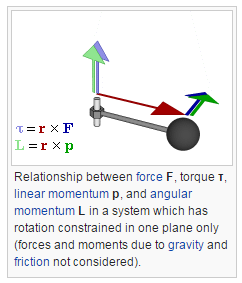
\includegraphics[width=0.3\textwidth]{torque}
  \end{center}
  \caption{}
  \label{fig:torque}
\end{wrapfigure}

Loosely speaking, \textit{torque} is a measure of the turning force on an object. \\ 

The magnitude of torque depends on 3 quantities: the force applied, the length of the lever arm connecting the axis to the point of force application, and the angle between the force vector and the lever arm (see Figure~\ref{fig:torque}). In symbols: \\
$\tau = r \times F$ \\
$\tau = \norm{r} \cdot \norm{F} sin \theta $ \\
$\tau$ - torque vector / magnitude of torque vector \\
r - displacement vector \\
F - force vector \\
$\theta$ - angle between the force vector and the lever arm vector

\clearpage

\subsection{Cross Product}
\textit{Algebraic Properties}

\begin{itemize}
    \item If $a \times b = 0$ then $a = 0$ or $b = 0$ or the sine between them is $0$ (they are parallel or antiparallel).
    \item The self cross product of a vector is the zero vector: \\ $a \times a = 0$
    \item The cross product is \textbf{anticommutative}:\\ $a \times b = - (b \times a)$
    \item It is \textbf{distributive} over addition:\\ $a \times (b+c) = a \times b + a \times c$
    \item It is \textbf{compatible with scalar multiplication}:\\ $(ra) \times b = a \times (rb) = r(a \times b)$
    \item It is \textbf{not associative} but satisfies the Jacobi identity:\\ $a \times (b \times c) + b \times(c \times a) + c \times(a \times b ) = 0$
\end{itemize}
